\chapter{Einleitung}
\label{cha:einleitung}

In dieser Arbeit werden die zentralen Eigenschaften von Microservices im Zusammenhang ihrer Skalierfähigkeit untersucht.
Im Mittelpunkt wird die Verteilung der Microservices behandelt und die gewonnen Kenntnisse sowohl in der Infrastruktur der Forschungsgruppe als auch der Infrastruktur des Kooperationspartners analysiert.
Des Weiteren wird auf den Entwicklungsprozess eingegangen, sodass die Skalierbarkeit der Microservices optimiert wird.

\section{Einführung in das Themengebiet}

\todo{Mehr auf die Verteilung der Services eingehen?}
\todo{Die CI/CD Pipeline einbeziehen?}

Onlinedienste wie bspw. Netflix, Spotify und Zalando möchten ihren Kunden eine globale und stetige Erreichbarkeit ihrer Anwendung bereitstellen.
Dies hat zur Folge, dass Nutzer solcher Onlinedienste eine hohe Erwartungshaltung gegenüber ebendieser Eigenschaften haben.
Die Dienste müssen in der Lage sein mehrere Millionen Nutzeranfragen bearbeiten zu können, ohne, dass dies zu einem Ausfall der Anwendung führt.
Im Mittelpunkt steht dabei die Skalierbarkeit der Anwendung, sodass die Ausfallzeit eines Services minimiert werden kann.
Insbesondere hat die Evolution der Softwarearchitektur von einer monolithischen Architektur zur Microservice-Architektur den Prozess der Skalierbarkeit angetrieben.
Neben den oben genannten Unternehmen setzen Amazon, Sound Cloud und Ebay ebenfalls auf die Microservice-Architektur, um die hohe Anzahl an Nutzeranfragen bearbeiten zu können.
Einer der Hauptvorteile ist, dass Microservices wiederverwendbare Funktionalität kapseln und dadurch unabhängig voneinander skaliert werden können.
Wird ein bestimmter Microservice einer Web-Anwendung stärker ausgelastet, so kann darauf reagiert werden und durch eine Anpassung der Infrastruktur der Microservice unterstützt werden.
Auf der einen Seite kann ein Rechner durch das Hinzufügen von Ressourcen wie bspw. Arbeitsspeicher oder einer Festplatte vertikal skaliert werden.
Auf der anderen Seite können weitere Rechner dem System hinzugefügt werden und somit die Auslastung des Microservices gesteuert werden.
Bei der Einhaltung der geforderten Eigenschaften nehmen die Werkzeuge Docker und Kubernetes eine zentrale Rolle ein.
Dabei ermöglicht Docker die Isolation des Microservices von der Hardware und sichert durch die Verwaltung von Abhängigkeiten einen konsistenten Zustand, der auf jeder Maschine hergestellt werden kann. 
Kubernetes dient zur Orchestrierung der Docker Container und abstrahiert diese.
Dadurch ist es Kubernetes möglich die Container selbst zu verwalten und bildet somit den integralen Bestandteil zur Skalierung von Microservices.
Die Werkzeuge ermöglichen nicht nur die Skalierung eines Microserivces, sondern auch dessen Verteilung.
Schwerpunkt dieser Arbeit ist die Bewertung von Microservices im Hinblick auf die Skalierbarkeit und die Ermittlung der wesentlichen Faktoren, die bereits im Entwicklungsprozess einen Einfluss auf die Skalierfähigkeit des Mircoservices haben.

\section{Fragestellungen}
Darstellung der in der Arbeit bearbeiteten Aspekte. Es bietet sich an, in diesem Abschnitt bereits die Grundlage für die Struktur der Gesamtarbeit (im Wesentlichen Kapitel 4 bis 4+n, siehe unten) zu legen.

\section{Beschreibung des Demonstrators}
Der Demonstrator dient dazu, die im vorhergehenden Abschnitt auf konzeptioneller Ebene eingeführten Fragestellungen anhand eines praktischen Beispiels zu verdeutlichen und eine Lösung aufzuzeigen.

\section{Gliederung der Arbeit}
\label{sec:gliederung}
In diesem Kapitel wird der Aufbau der Arbeit in Form der Kapitelstruktur aufgezeigt. Fol-gende Kapitelstruktur wird empfohlen:

\subsection*{Kapitel 2: Grundlagen}



Dieses Kapitel beinhaltet Informationen, die zum grundlegenden Verständnis der Inhalte der Arbeit erforderlich sind. Die Informationen werden weitestgehend "wertfrei" darge-stellt. Beispiele sind:...

\subsection*{Kapitel 3: Stand der Technik}

In dieses Kapitel fließen ganz wesentlich die Ergebnisse der Literaturanalyse ein. Es bietet sich an, die in der Einleitung eingeführte Struktur hier wieder aufzugreifen.

Im Gegensatz zu Kapitel 2 werden die Inhalte dieses Kapitels in einer argumentativen und wertenden Form dargestellt.

\subsection*{Kapitel 4: Inhalt}

Kapitel 4 bis 4+n sind die zentralen konzeptionellen Kapitel der Arbeit, in denen die er-zielten Ergebnisse beschrieben werden.

\subsection{Latex-Vorlagen}

\subsection{Zitate}
\label{subsec:zitate}
Der Demonstrator nutzt meist Komponenten, die bereit sin früheren Arbeiten bei \gls{CM} entwickelt wurden.
\begin{quote}
\textit{``A microservice is a cohesive, independent process interacting via messages``}
\end{quote}
\begin{quote}
\textit{``fictive book quote.'', \cite[S.~99]{Be02}}
\end{quote}

\subsection{Grafiken}
Einfügen von Grafiken und referenzieren der Abbildung \ref{fig:lehre}.
\begin{figure}[h]
	\centering
	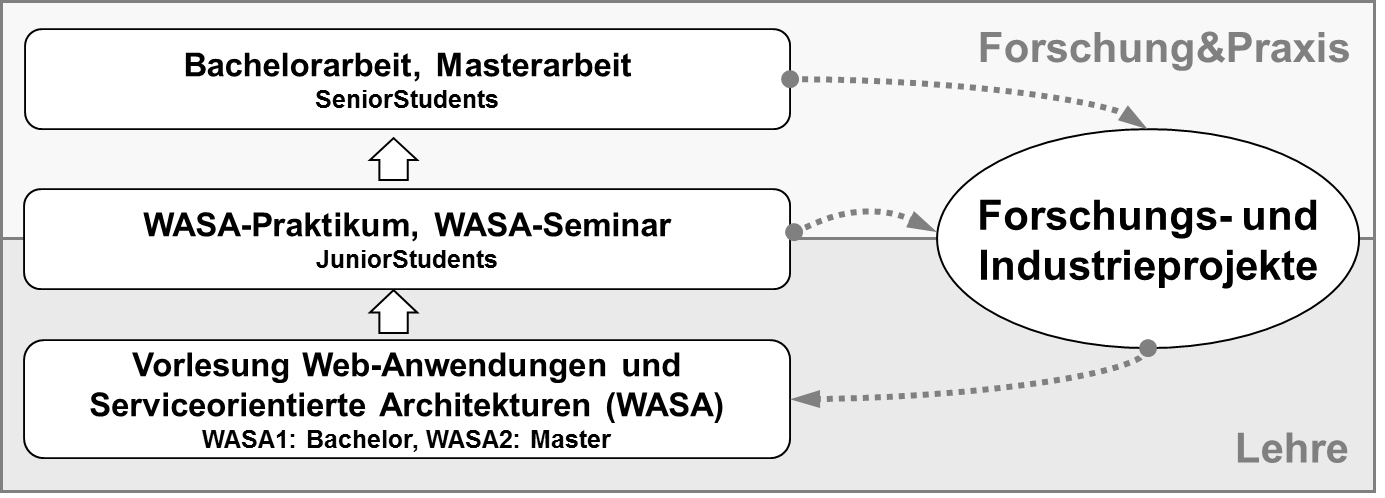
\includegraphics[width=0.8\textwidth]{images/lehre_kreislauf.png}
	\caption{Lehre-Forschung \& Praxis-Kreislauf}
	\label{fig:lehre}
\end{figure}

\begin{table}
	\centering
	\begin{tabular}{ | l | p{7cm} | }
		\hline
		ServiceGroup & Dienstleistung \\
		\hline
		 CoreServiceGroup & Campus-Informationen und Navigation \\
	 	\hline
	 	SCbInfoServiceGroup (SCbSG) & Hörsaal-Informationen für Studierende mit Beeinträchtigung \\
	 	\hline
	 	 StudAdviceTicket (StuSG) & Studierendenberatungs-Anmeldung \\
	 	\hline
	 	WorkspaceServiceGroup (WorSG) & Arbeitsplatz-Suche und -Reservierung \\
	 	\hline
	 	BaMaThesisAdminSG (BaMSG) & Abschlussarbeitenverwaltung \\
	 	\hline
	\end{tabular}
	\caption{ServiceGroups in SmartCampus}
	\label{tab:smartcampus-servicegroups}
\end{table}

\subsection{Quellcode}
\vspace{0.5cm}
\begin{lstlisting}[caption = {Vorlage für eine Story und Szenarien nach BDD}, label = {lst:bdd-stories-szenarien-template}, style = kit-cm, language = Gherkin]
Title (one line describing the story)
 
Narrative:
As a [role]
I want [feature]
So that [benefit]
 
Acceptance Criteria: (presented as Scenarios)
 
Scenario 1: Title
Given [context]
  And [some more context]...
When  [event]
Then  [outcome]
  And [another outcome]...
 
Scenario 2: ...
\end{lstlisting}

